%%==============================================================================
%% VHD-FL: Verifiable Hierarchical Federated Learning with Distributed Key
%% Generation for UAV Swarms
%%
%% IEEE Transactions double-column manuscript (10 pt, journal).
%% Build:  latexmk -pdf main.tex
%%   (or)  pdflatex main -> bibtex main -> pdflatex main -> pdflatex main
%%
%% Section files:
%%   abstract.tex  introduction.tex  related_work.tex  preliminaries.tex
%%   scheme.tex    algorithm_design.tex  security.tex  evaluation.tex
%%   conclusion.tex
%%
%% Author photographs are kept in ./authors and figures (self-contained
%% diagrams/plots) are generated inline with TikZ/pgfplots, so the project
%% compiles without any external figure dependency.
%%==============================================================================
\documentclass[10pt,journal]{IEEEtran}

%%------------------------------------------------------------------------------
%% Core math
%%------------------------------------------------------------------------------
\usepackage{amsmath,amssymb,amsfonts}
\usepackage{amsthm}
\usepackage{mathtools}
\usepackage{bm}

%%------------------------------------------------------------------------------
%% Graphics, colour, TikZ / pgfplots (self-contained figures)
%%------------------------------------------------------------------------------
\usepackage{graphicx}
\graphicspath{{figures/}{authors/}}
\usepackage{xcolor}
\usepackage{tikz}
\usetikzlibrary{shapes,arrows,arrows.meta,positioning,calc,fit,backgrounds,%
                patterns,decorations.pathreplacing,chains,matrix}
\usepackage{pgfplots}
\pgfplotsset{compat=1.18}
\usepgflibrary{shapes.geometric}

%%------------------------------------------------------------------------------
%% Tables
%%------------------------------------------------------------------------------
\usepackage{booktabs}
\usepackage{colortbl}
\usepackage{tabularx}
\usepackage{array}
\usepackage{multirow}
\usepackage{caption}
\usepackage{subcaption}

%%------------------------------------------------------------------------------
%% References, lists, symbols
%%------------------------------------------------------------------------------
\usepackage{cite}
\usepackage{enumitem}
\usepackage{pifont}
\newcommand{\cmark}{\ding{51}}
\newcommand{\xmark}{\ding{55}}

%%------------------------------------------------------------------------------
%% Algorithms (algorithm2e, ruled)
%%------------------------------------------------------------------------------
\usepackage[ruled,linesnumbered,commentsnumbered]{algorithm2e}

%%------------------------------------------------------------------------------
%% Palette (muted, print-friendly)
%%------------------------------------------------------------------------------
\definecolor{WorkerBlue}{RGB}{60,110,170}
\definecolor{HeadTeal}{RGB}{40,135,120}
\definecolor{ServerRed}{RGB}{185,75,70}
\definecolor{CommentBlue}{RGB}{0,80,160}
\definecolor{MaskGreen}{RGB}{50,135,85}
\definecolor{CipherPurple}{RGB}{110,80,150}
\definecolor{HashGold}{RGB}{180,140,45}
\definecolor{LightGray}{RGB}{245,245,245}

%%------------------------------------------------------------------------------
%% Algorithm2e style
%%------------------------------------------------------------------------------
\newcommand{\cmtfont}{\footnotesize\color{CommentBlue}}
\newcommand{\cmtmarker}{$\triangleright$~}
\SetCommentSty{cmtfont}
\SetKwComment{tcp}{\cmtmarker}{}
\SetKwComment{tcc}{\cmtmarker}{}
\SetKwInput{KwInput}{Input}
\SetKwInput{KwOutput}{Output}
\SetKwInput{KwParam}{Parameter}
\DontPrintSemicolon
\SetAlgoNlRelativeSize{0}

%%------------------------------------------------------------------------------
%% Theorem-like environments
%%------------------------------------------------------------------------------
\newtheorem{theorem}{Theorem}
\newtheorem{lemma}{Lemma}
\newtheorem{corollary}{Corollary}
\newtheorem{definition}{Definition}
\newtheorem{assumption}{Assumption}
\newtheorem{remark}{Remark}

%%------------------------------------------------------------------------------
%% Unified mathematical notation
%%   (every symbol is also defined in the Notation Table, preliminaries.tex)
%%------------------------------------------------------------------------------
% Number systems / rings
\newcommand{\R}{\mathbb{R}}
\newcommand{\Z}{\mathbb{Z}}
\newcommand{\N}{\mathbb{N}}
\newcommand{\E}{\mathbb{E}}
\newcommand{\Rq}{\mathcal{R}_q}
\newcommand{\Rp}{\mathcal{R}_p}
\newcommand{\Rring}{\mathcal{R}}
\newcommand{\U}{\mathcal{U}}
\DeclareMathOperator*{\argmax}{arg\,max}

% Cryptographic primitives
\DeclareMathOperator{\Enc}{Enc}
\DeclareMathOperator{\Dec}{Dec}
\DeclareMathOperator{\Eval}{Eval}
\DeclareMathOperator{\Sign}{Sign}
\DeclareMathOperator{\Verify}{Verify}
\DeclareMathOperator{\KeyGen}{KeyGen}
\DeclareMathOperator{\HH}{HH}          % homomorphic hash
\newcommand{\negl}{\operatorname{negl}}

% Ciphertext / message shorthand
\newcommand{\ct}{\mathsf{ct}}
\newcommand{\sk}{\mathsf{sk}}
\newcommand{\vk}{\mathsf{vk}}
\newcommand{\pk}{\mathsf{pk}}
\newcommand{\bbar}{\bar{b}}
\newcommand{\ebar}{\bar{e}}
\newcommand{\mglob}{M}
\newcommand{\Share}[1]{[s]_{#1}}       % threshold share of group secret

% Small helpers
\newcommand{\qedblack}{\hfill$\blacksquare$}
\newcommand{\round}{\ell}               % communication round index
\newcommand{\thr}{\tau}                 % threshold

%% hyperref must be loaded last
\usepackage[colorlinks=false,pdfborder={0 0 0}]{hyperref}

%%==============================================================================
\begin{document}
%%==============================================================================

\title{VHD-FL: Verifiable Hierarchical Federated Learning with Distributed Key Generation for UAV Swarms}

\author{
    Zhongyang~Shi,
    Hong~Zhong,
    Qingyang~Zhang,
    Ke~Cheng,
    Fengqun~Wang,
    and~Jie~Cui
    \IEEEcompsocitemizethanks{
        \IEEEcompsocthanksitem Z. Shi, H. Zhong, Q. Zhang, F. Wang, and J. Cui are with the Key Laboratory of Intelligent Computing and Signal Processing of the Ministry of Education, School of Computer Science and Technology, Anhui University, Hefei 230039, China, and also with the Anhui Engineering Laboratory of IoT Security Technologies, Anhui University, Hefei 230039, China (e-mail: zhongh@ahu.edu.cn; cuijie@mail.ustc.edu.cn). (Corresponding author: Hong Zhong.)
        \IEEEcompsocthanksitem K. Cheng is with the School of Computer Science and Technology, Xidian University, Xi'an 710126, China, and also with the Shaanxi Key Laboratory of Network and System Security, Xi'an 710071, China (e-mail: chengke@xidian.edu.cn).
    }
}

\maketitle

%%---- Front matter -----------------------------------------------------------
%%==============================================================================
%% Abstract and keywords
%%==============================================================================
\begin{abstract}
Federated learning (FL) over hierarchical unmanned aerial vehicle (UAV) swarms allows collaborative model training across worker UAVs, cluster-head UAVs, and a cloud server without relocating raw sensing data. Securing this architecture, however, imposes a set of coupled constraints that existing protocols do not jointly resolve: MCU-class worker UAVs cannot afford the number-theoretic transform underlying homomorphic encryption, no trusted authority is available to issue a group key, and the cluster-heads and cloud are mutually untrusted, may collude, and may tamper with encrypted inputs, fabricate the aggregation, or submit erroneous decryption shares. We present \textsc{VHD-FL}, a verifiable hierarchical FL framework that reconciles these constraints without introducing a new trusted entity. A cluster-head-layer distributed key generation produces the group key with zero participation by worker UAVs and zero key shares held by the cloud. A three-blind outsourced encryption protocol reuses a neighboring cluster-head as the third mask holder, yielding a 3-out-of-3 additive secret sharing that tolerates collusion among any two mask holders. Three-layer verifiability---an encryption zero-knowledge proof, a homomorphic hash over the aggregation, and a decryption proof---detects tampering, forged aggregation, and incorrect partial decryption against a malicious cloud. Experiments on MNIST, CIFAR-10, and FEMNIST show that \textsc{VHD-FL} matches plaintext FedAvg accuracy while reducing per-round worker cost to a single modular subtraction and one EdDSA signature, and that it tolerates up to $\tau-1$ colluding cluster-heads and arbitrary worker dropouts.
\end{abstract}

\begin{IEEEkeywords}
Federated learning, unmanned aerial vehicles, distributed key generation, homomorphic encryption, verifiability, collusion resistance.
\end{IEEEkeywords}

%%==============================================================================
%% Section I: Introduction
%%==============================================================================
\section{Introduction}
\label{sec:introduction}

\begin{figure}[t]
  \centering
  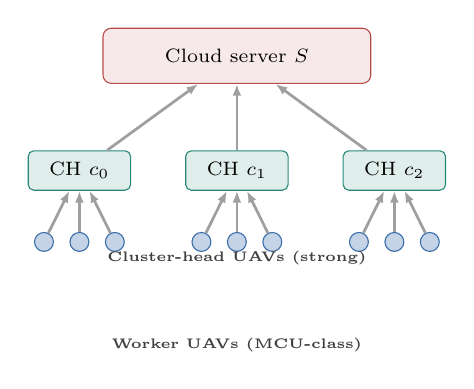
\begin{tikzpicture}[font=\tiny,
    wnode/.style={circle,inner sep=0pt,minimum size=2.4mm,fill=WorkerBlue!30,draw=WorkerBlue},
    hnode/.style={rectangle,rounded corners=2pt,inner sep=1.5pt,minimum height=5mm,
                  minimum width=13mm,fill=HeadTeal!15,draw=HeadTeal},
    snode/.style={rectangle,rounded corners=3pt,inner sep=2pt,minimum height=7mm,
                  minimum width=34mm,fill=ServerRed!12,draw=ServerRed},
    flow/.style={-{Latex[length=1.5mm]},gray!75,line width=0.35mm}]
    % --- Cloud ---
    \node[snode] (S) {\scriptsize Cloud server $S$};
    % --- Cluster heads ---
    \foreach \i/\x in {0/-20,1/0,2/20}{
      \node[hnode] (H\i) at ($(S.south)+( \x mm,-11mm)$) {\scriptsize CH $c_{\i}$};
    }
    % --- Workers ---
    \foreach \i in {0,1,2}{
      \foreach \k/\dx in {0/-4.5,1/0,2/4.5}{
        \node[wnode] (w\i\k) at ($(H\i.south)+( \dx mm,-6.5mm)$) {};
      }
    }
    % --- Links ---
    \foreach \i in {0,1,2}{
      \draw[flow] (H\i) -- (S);
      \foreach \k in {0,1,2}{\draw[flow] (w\i\k) -- (H\i);}
    }
    % --- Tier labels ---
    \node[HeadTeal,align=center,font=\tiny] at ($(H1)+(0,-1.5mm)$) {};
    \node[anchor=north,font=\tiny,text=black!75] at ($(S.south)+(0,-20mm)$)
      {\textbf{Cluster-head UAVs (strong)}};
    \node[anchor=north,font=\tiny,text=black!75] at ($(S.south)+(0,-31mm)$)
      {\textbf{Worker UAVs (MCU-class)}};
  \end{tikzpicture}
  \caption{Three-tier hierarchical FL over a UAV swarm. MCU-class worker UAVs are grouped into clusters, each governed by a capable cluster-head (CH) that performs the cryptographic workload and pre-aggregation; the cluster-heads connect to a cloud server that performs global aggregation and coordinates verification.}
  \label{fig:hierarchy}
\end{figure}

\IEEEPARstart{U}{nmanned} aerial vehicle (UAV) swarms are increasingly deployed for disaster response, environmental monitoring, reconnaissance, and intelligent surveillance, in which a fleet of small, battery-powered aircraft collaborates to sense and act over a target area. Training a shared perception or decision model across the fleet is essential, yet the raw imagery, telemetry, and location traces are both volume-heavy and privacy-sensitive, which makes centralizing them impractical. Federated learning (FL) offers a natural fit: each vehicle trains locally on its own data and exchanges only model updates, so that raw samples never leave the device~\cite{bonawitz2019towards}. Because a flat, fully connected topology does not scale to large fleets, practical deployments organize the aircraft into a three-tier hierarchy in which worker UAVs are grouped into clusters governed by a more capable cluster-head UAV, and the cluster-heads in turn connect to a cloud server. Hierarchical aggregation over this topology reduces both the number of long-range links and the energy cost incurred at the weakest nodes~\cite{liu2020hierfavg},~\cite{wang2021rflha}, and it has become the standard structure for UAV-based collaborative learning~\cite{ahmed2025uav},~\cite{nagarajan2025drone}.

Exchanging model updates, however, does not by itself preserve privacy. A broad line of gradient-inversion and reconstruction attacks demonstrates that, from a single update, an adversary can recover much of the underlying training data~\cite{zhu2019deep},~\cite{geiping2020inverting},~\cite{zhao2020idlg}, and recent studies show that these attacks remain effective against modern architectures~\cite{guo2025exploring}. In a swarm, the cloud and even peer cluster-heads occupy strong vantage points and are therefore realistic adversaries. Three families of countermeasures are commonly adopted. Differential privacy (DP)~\cite{mcmahan2017learning} injects calibrated noise but incurs a utility trade-off; secure aggregation built on secure multi-party computation~\cite{bonawitz2017practical} masks pairwise updates; and homomorphic encryption (HE)~\cite{gentry2009fully} allows the cloud to aggregate ciphertexts without learning any individual update. HE is particularly attractive for secure aggregation, and the Cheon--Kim--Kim--Song (CKKS) scheme~\cite{cheon2017ckks}, which is built on the ring learning-with-errors (RLWE) problem~\cite{lyubashevsky2010ideal}, supports approximate arithmetic and is well matched to real-valued neural-network updates.

Deploying HE on a swarm exposes a sharp resource asymmetry. The dominant cost of CKKS encryption is a number-theoretic transform over a large polynomial ring, whose memory and energy footprint are prohibitive for the MCU-class processors that power small worker UAVs, while the larger cluster-heads can perform it. Outsourcing encryption to a cluster-head is the natural remedy, but it immediately raises two new problems. First, the cluster-head and cloud that mediate the outsourced computation are themselves untrusted, so a plaintext update handed to them is exposed. Second, conventional HE relies on a globally shared key that would allow any one intermediary to decrypt every update; existing outsourcing protocols therefore introduce a key distribution center or a trusted authority, and some additionally rely on a trusted execution environment~\cite{li2025fedphe},~\cite{wu2025esafl},~\cite{yuan2026fedout},~\cite{cai2023secfed}. In fielded UAV missions, however, no such trusted infrastructure is available.

Removing the trusted anchor is not sufficient, because two structural vulnerabilities remain. On the one hand, intermediaries are not merely curious but potentially malicious: a cluster-head may encrypt a modified plaintext and thereby poison the global model, and the cloud may fabricate an aggregate, selectively discard updates, or request the decryption of a chosen individual. On the other hand, the threat model explicitly permits the cluster-heads and cloud to collude, which is fatal to a naive two-party outsourcing design in which one party sees the blinded plaintext and the other holds a single masking factor, since their two views reconstruct the update. Prior verifiable protocols either stop at decryption-time verification without an inclusion proof~\cite{bouamama2025vesafl}, or add a dedicated masking server that is not part of the fixed three-tier topology. Three challenges therefore emerge:

\begin{itemize}[leftmargin=*,topsep=2pt,itemsep=1pt]
  \item \textbf{C1: Key establishment without trust.} How can a group decryption key be established without a trusted authority when worker UAVs cannot participate in key generation and the cloud must not be able to decrypt alone?
  \item \textbf{C2: Entity-free collusion-resistant outsourcing.} How can encryption be outsourced to a cluster-head while hiding the update from the cluster-head and cloud even when they collude, using only the entities already present in the three-tier hierarchy?
  \item \textbf{C3: End-to-end verifiability and dropout tolerance.} How can encryption, aggregation, and decryption be made publicly verifiable against a malicious cloud and corrupted cluster-heads while tolerating the frequent worker and cluster-head dropouts of wireless swarms?
\end{itemize}

We address these questions with \textsc{VHD-FL}. To answer C1, the cluster-heads run a distributed key generation (DKG) to establish a group key, and the resulting secret is shared among the cluster-heads through a threshold verifiable secret-sharing scheme; worker UAVs take no part in key generation and the cloud holds no share, so the cloud alone cannot decrypt. To answer C2, each worker masks its update with a blinding factor split into three additive shares and delivers them to its own cluster-head, the cloud, and a neighboring cluster-head arranged in a ring. The neighboring cluster-head is an existing strong node, so no new entity is introduced, and the three shares form a 3-out-of-3 secret sharing that resists collusion between any two holders. To answer C3, \textsc{VHD-FL} enforces three-layer verifiability: a zero-knowledge proof binds each ciphertext to the blinded plaintext, a homomorphic hash detects a forged aggregate or selective omission, and a further proof validates every partial decryption; threshold reconstruction and zero ciphertexts tolerate dropouts.

The main contributions are summarized as follows:
\begin{itemize}[leftmargin=*,topsep=2pt,itemsep=1pt]
  \item We design a \textbf{trust-anchor-free cluster-head DKG} that integrates a threshold verifiable secret sharing into the aggregation key. Worker UAVs contribute nothing to key generation and the cloud holds no share, yielding collusion-resistant threshold decryption without a trusted authority.
  \item We propose \textbf{three-blind outsourced encryption} that reuses a neighboring cluster-head as the third mask holder. It realizes 3-out-of-3 additive secret sharing, resists collusion between any two mask holders without adding an entity, and reduces per-round worker work to a single modular subtraction plus one lightweight signature.
  \item We establish \textbf{three-layer verifiability}---encryption zero-knowledge proofs, a homomorphic hash over the aggregation, and decryption proofs---against a malicious cloud and corrupted cluster-heads. We prove the corresponding privacy, verifiability, and dropout-tolerance properties, and experiments on MNIST, CIFAR-10, and FEMNIST show that \textsc{VHD-FL} matches plaintext FedAvg accuracy while substantially reducing worker and communication overhead.
\end{itemize}

The remainder of this paper is organized as follows. Section~\ref{sec:related} reviews related work. Section~\ref{sec:preliminaries} introduces the system model, threat model, cryptographic building blocks, and notation. Section~\ref{sec:scheme} details the \textsc{VHD-FL} scheme, and Section~\ref{sec:algorithms} presents the algorithms. Section~\ref{sec:security} gives the security analysis, Section~\ref{sec:evaluation} reports the performance evaluation, and Section~\ref{sec:conclusion} concludes the paper and discusses future directions.

%%==============================================================================
%% Section II: Related Work
%%==============================================================================
\section{Related Work}
\label{sec:related}

We review five lines of research that meet the requirements of a UAV swarm: homomorphic-encryption-based FL, secure aggregation, hierarchical and UAV FL, distributed key generation, and verifiable FL against collusion.

\textbf{Homomorphic-Encryption-Based FL.} HE permits computation directly on ciphertexts and therefore offers the strongest cryptographic guarantee for private aggregation. Single-key CKKS constructions such as FedSHE~\cite{pan2024fedshe} and FedPHE~\cite{li2025fedphe} exploit approximate arithmetic and ciphertext packing, but a globally shared key lets any key holder decrypt every update. Multi-key HE removes this exposure by allowing independent client keys: Chen et al.~\cite{chen2019efficient} introduced efficient packed multi-key encryption, and ESAFL~\cite{wu2025esafl} together with the construction of Wu et al.~\cite{wu2025secure} refine packing and one-step decryption for cross-silo settings. To relieve weak clients, FedOut~\cite{yuan2026fedout} and CDKS-LSS~\cite{wang2026cdks} outsource encryption to an intermediary and combine MKHE with secret sharing, while EVMKA~\cite{yang2026evmka} adds verifiable multi-key aggregation. These systems nevertheless retain a common limitation: the single-key schemes leave a holder able to decrypt, whereas the outsourcing systems rely on a key distribution center or a trusted authority and assume the intermediary is only semi-honest. None resists a malicious intermediary jointly with collusion, and the encryption cost is displaced rather than eliminated without a trust anchor.

\textbf{Secure Aggregation.} Masking-based secure aggregation avoids the cost of HE. Bonawitz et al.~\cite{bonawitz2017practical} established the practical blueprint using pairwise masking with dropout recovery; LightSecAgg~\cite{so2022lightsecagg} and $\lambda$-SecAgg~\cite{ergun2025lambda} reduce per-client work through encoded and partially frozen masks, Flamingo~\cite{ma2023flamingo} supports multi-round single-server aggregation, and single-setup protocols~\cite{sultan2025single} provide forward and backward secrecy. TEE-aided systems such as SecFed~\cite{cai2023secfed} and Lancelot~\cite{jiang2024lancelot} provide hardware-rooted guarantees. These protocols remain vulnerable to adversarial server selection, which is only partially addressed by Lotto~\cite{jiang2024lotto}; more importantly, they authenticate the aggregate but do not bind a ciphertext to its underlying plaintext nor verify the decryption shares, and the TEE variants require hardware that is absent on small UAVs.

\textbf{Hierarchical and UAV FL.} Hierarchical FL inserts an aggregation tier between clients and the cloud. Liu et al.~\cite{liu2020hierfavg} analyzed Client-Edge-Cloud hierarchical FL (HierFAVG), Wang et al.~\cite{wang2021rflha} introduced resource-efficient hierarchical aggregation, and heterogeneous frameworks that balance completion time and accuracy have been reported in~\cite{wang2026heterogeneous}; partial-error feedback~\cite{xin2026safe} and sporadic personalization~\cite{rahman2026tackling} further address heterogeneous clients. UAV-specific swarm frameworks and surveys examine collaborative training across fleets~\cite{nagarajan2025drone},~\cite{ahmed2025uav}. This line of work primarily targets convergence, latency, and energy, and it generally assumes the aggregation tier and cloud are honest; it does not address how MCU-class worker UAVs produce encrypted updates, how the aggregation key is generated without a trusted authority, or how a malicious cloud can be detected.

\textbf{Distributed Key Generation.} Shamir secret sharing~\cite{shamir1979} underlies threshold cryptography, and Feldman verifiable secret sharing (VSS)~\cite{feldman1987} makes shares publicly checkable; Pedersen VSS~\cite{pedersen1991} adds information-theoretic privacy for the shared value, and Gennaro et al.~\cite{gennaro2007dkg} formalized secure DKG for discrete-log cryptosystems. These are general-purpose primitives over discrete-log groups that are not directly integrated with the RLWE-based encryption used for FL. Adopting them directly would additionally require weak worker UAVs to participate in key generation, which is infeasible; how to confine a DKG to the strong cluster-head tier and couple it to an RLWE aggregator remains unexplored.

\textbf{Verifiable FL and Collusion Resistance.} Verifiable FL aims to detect a malicious server or corrupted clients. VeSAFL~\cite{bouamama2025vesafl} combines short signatures with a verifiable sharing scheme, and dual-verifiable FL~\cite{cui2026dualverifiable} uses vector commitments and a semi-trusted verification cluster against collusion. Byzantine-robust systems such as~\cite{dong2023privacy},~\cite{cao2024srfl}, and~\cite{jiang2024lancelot} tolerate model poisoning. VeSAFL verifies decryption without an inclusion proof, while the dual-verifiable design introduces a separate verification cluster that amounts to a new entity; the Byzantine-robust systems assume an honest server and therefore do not protect against a malicious cloud that forges the aggregate. To our knowledge, no existing framework simultaneously provides trust-anchor-free key generation, collusion-resistant outsourced encryption, and end-to-end three-layer verification within the fixed worker--cluster-head--cloud hierarchy, which is the gap that \textsc{VHD-FL} is designed to close. Table~\ref{tab:capability} summarizes the comparison.

\begin{table*}[t]
\centering
\caption{Capability Comparison of VHD-FL with Representative Privacy-Preserving FL Schemes}
\label{tab:capability}
\scriptsize
\setlength{\tabcolsep}{4.2pt}
\renewcommand{\arraystretch}{1.2}
\begin{tabular}{@{}lccccccc@{}}
\toprule
Scheme & TTP-free & No NTT & Collusion res. & Ver. enc. & Ver. agg. & Ver. dec. & Dropout \\
\midrule
FedOut~\cite{yuan2026fedout}    & \xmark & \cmark & \xmark & \xmark & \xmark & Partial & \xmark \\
CDKS-LSS~\cite{wang2026cdks}    & \xmark & \cmark & Partial & \xmark & \xmark & \xmark & Partial \\
ESAFL~\cite{wu2025esafl}        & \xmark & \xmark & \xmark & \xmark & \xmark & \xmark & \xmark \\
FedPHE~\cite{li2025fedphe}      & \xmark & \xmark & \xmark & \xmark & \xmark & \xmark & Partial \\
VeSAFL~\cite{bouamama2025vesafl}& \xmark & \cmark & Partial & \xmark & \cmark & \cmark & Partial \\
\textbf{VHD-FL}                 & \cmark & \cmark & \cmark & \cmark & \cmark & \cmark & \cmark \\
\bottomrule
\end{tabular}
\end{table*}


%%---- Preliminaries ----------------------------------------------------------
%%==============================================================================
%% Section III: Preliminaries (notation table, system/threat model, primitives)
%%==============================================================================
\section{Preliminaries}
\label{sec:preliminaries}

\subsection{Notation}
Table~\ref{tab:notation} lists the symbols used throughout the paper. Acronyms are defined at first use, and every mathematical symbol is defined in the table, so subsequent sections do not repeat its definition.

\begin{table}[t]
\centering
\caption{Summary of Key Notation}
\label{tab:notation}
\footnotesize
\setlength{\tabcolsep}{2.5pt}
\renewcommand{\arraystretch}{1.12}
\begin{tabularx}{\columnwidth}{@{}>{\raggedright\arraybackslash}p{0.27\columnwidth} >{\raggedright\arraybackslash}X@{}}
\toprule
\textbf{Notation} & \textbf{Description} \\
\midrule
\multicolumn{2}{@{}l}{\textit{System and Hierarchy}}\\
$\lambda,n,q,\Delta$ & Security parameter, ring dimension, modulus, CKKS scale \\
$N,M,\tau$ & Numbers of worker UAVs, cluster-heads, and threshold \\
$G_c,N_c,c'$ & Worker set of cluster $c$, its size, neighbor head \\
$\ell,T$ & Communication round index and total rounds \\
$S$ & Cloud server \\
\midrule
\multicolumn{2}{@{}l}{\textit{Keys and Shares}}\\
$s_c,b_c$ & CH $c$ secret contribution and public component \\
$s,\bar{b}$ & Group secret and group public key \\
$[s]_c,pk_c^*$ & CH $c$ threshold share and share public key \\
$sk_i^{\mathrm{sig}},vk_i^{\mathrm{sig}}$ & Worker EdDSA signing and verification keys \\
\midrule
\multicolumn{2}{@{}l}{\textit{Updates, Masks, and Hash}}\\
$m_i,m_i'$ & Worker update and blinded update \\
$r_i^{(c)},r_i^{(s)},r_i^{(c')}$ & Three mask shares; $r_i$ is their sum \\
$h_i,\sigma_i$ & Homomorphic hash and worker signature \\
\midrule
\multicolumn{2}{@{}l}{\textit{Ciphertexts, Proofs, and Crypto}}\\
$ct_i',ct^{(c)},ct_{\mathrm{glob}}$ & Individual, cluster, and global ciphertexts \\
$v_i,e_{i,0},e_{i,1}$ & Encryption randomizer and error terms \\
$D_c,\lambda_c$ & Partial decryption and Lagrange coefficient \\
$\pi_i^{\mathrm{enc}},\pi_c$ & Encryption and decryption NIZKs \\
$a,\chi_s,\chi_e$ & Public polynomial, key and error distributions \\
$\mathcal{R}_q,\mathcal{R}_p,\mathrm{negl}(\cdot)$ & Rings and negligible function \\
\bottomrule
\end{tabularx}
\end{table}

\subsection{Hierarchical FL and System Model}
\label{subsec:systemmodel}
We consider a three-tier hierarchical FL system. The $N$ worker UAVs are partitioned into $M$ disjoint clusters $G_1,\ldots,G_M$, with $N_c=|G_c|$ and $\sum_{c=1}^{M}N_c=N$. Each cluster is managed by one cluster-head UAV, and the $M$ heads connect to a cloud server. Worker $i$ holds a local dataset $\mathcal{D}_i$ and a model $w\in\mathbb{R}^{d}$. At round $\ell$, a worker performs local stochastic gradient descent to obtain an update $m_i$; the head pre-aggregates within the cluster, and the cloud aggregates the $M$ cluster results. The correct plaintext aggregate is
\begin{equation}
  \label{eq:plaintext-agg}
  \mglob=\sum_{i=1}^{N} m_i .
\end{equation}
Worker $i$ derives its update through local stochastic gradient descent over $E$ local epochs,
\begin{equation}
  \label{eq:local-update}
  m_i = w_{\ell-1}-w_i^{(E)},\qquad
  w_i^{(k+1)} = w_i^{(k)} - \eta_{\ell}\nabla\mathcal{L}(w_i^{(k)};\mathcal{B}_i),
\end{equation}
where $\mathcal{B}_i$ is a local minibatch and $\mathcal{L}$ the empirical loss. The data are heterogeneous: the class proportion vector $p_k$ of worker $k$ follows $p_k\sim\mathrm{Dir}(\alpha)$, and smaller $\alpha$ yields a more skewed partition.

We use unweighted aggregation for clarity; dataset-size weights $p_i$ can be absorbed by replacing each $m_i$ with $p_i m_i$.

The four role classes are as follows:
\begin{itemize}[leftmargin=*,topsep=2pt,itemsep=1pt]
  \item \textbf{Worker UAV $i$} ($N$, MCU-class, no NTT): local training, one-time pad blinding, sampling of three mask shares, a linear homomorphic hash, and an EdDSA signature.
  \item \textbf{Cluster-head UAV $c$} ($M$, strong): outsourced encryption, NIZK proofs, verifiable secret sharing, intra-cluster pre-aggregation, and partial decryption; it holds one share of the group secret.
  \item \textbf{Neighbor cluster-head $c'$} ($M$, strong): the ring neighbor $c'=(c+1)\bmod M$, which holds the third mask share and has the same capabilities as a head.
  \item \textbf{Cloud server $S$} ($1$, strong): aggregation and verification coordination, including threshold-decryption interpolation; it holds no key share.
\end{itemize}

\subsection{Threat Model and Security Goals}
\label{subsec:threat}
We make the following adversarial assumptions.
\begin{itemize}[leftmargin=*,topsep=2pt,itemsep=1pt]
  \item \textbf{Cloud server.} The cloud is \emph{malicious}: it may fabricate the aggregate, selectively discard updates, tamper with the downlink model, and selectively request the decryption of a chosen individual.
  \item \textbf{Cluster-heads.} Heads are \emph{semi-honest but curious} and corruptible; any coalition of at most $\tau-1$ heads, including a coalition with the cloud, cannot reconstruct the group secret.
  \item \textbf{Worker UAVs.} In the baseline model workers are honest-but-curious and may drop out arbitrarily. In the extended model, a malicious worker may upload any update and a captured worker is fully controlled by the attacker.
  \item \textbf{Mask holders.} Of the three holders of a blinded update, any two that collude cannot recover the update (3-out-of-3).
  \item \textbf{Channels and trust.} No trusted authority exists. The three mask shares are carried over independent secure channels; all other traffic is public.
\end{itemize}
Accordingly, \textsc{VHD-FL} targets four security goals: \emph{G1}, worker privacy against collusion; \emph{G2}, secrecy of the group decryption key against a threshold coalition; \emph{G3}, end-to-end verifiability of encryption, aggregation, and decryption against a malicious cloud; and \emph{G4}, tolerance of arbitrary worker and cluster-head dropouts.

We formalize these goals with two standard games. In the \emph{privacy game}, the adversary chooses two updates $m_0,m_1$, receives the transcript produced for a uniformly hidden bit $b$, and outputs a guess; the protocol is private if its distinguishing advantage is $\negl(\lambda)$. In the \emph{verifiability game}, the adversary controls the cloud and corrupted intermediaries and attempts to make the verifier accept an aggregate different from the honest one; the protocol is verifiable if this success probability is $\negl(\lambda)$. Section~\ref{sec:security} establishes both games and the dropout property.

\subsection{Ring Learning with Errors and CKKS}
\label{subsec:rlwe}
Let $R=\mathbb{Z}[X]/(X^n+1)$ be the cyclotomic ring for a power-of-two $n$, with residue ring $\mathcal{R}_q=R/qR$, and let $\chi_s$ and $\chi_e$ output small polynomials. The \emph{RLWE assumption} states that pairs $(a,b)$ with $a\leftarrow\mathcal{U}(\mathcal{R}_q)$, $s\leftarrow\chi_s$, and $b=[-as+e]_q$ for $e\leftarrow\chi_e$ are computationally indistinguishable from uniform pairs in $\mathcal{R}_q^2$~\cite{lyubashevsky2010ideal}.

CKKS~\cite{cheon2017ckks} maps a real vector to a plaintext polynomial through an isometric isomorphism $\varphi:R\to\mathbb{C}^{n/2}$ and a scaling factor $\Delta$, packing $n/2$ values into one ciphertext (SIMD). It is additively homomorphic, which is all that secure aggregation requires. Recent diagonal packing improves the slot layout for matrix and sparse vectors~\cite{lee2026hydia},~\cite{deryabin2026packing}, and refined modular approximation lowers the noise~\cite{zhang2026efficient}. We use its standard public-key form. The public key is $(\bar b,a)$ with $\bar b=-as+\bar e$; to encrypt a message $m$, sample $v\leftarrow\chi_s$ and $e_0,e_1\leftarrow\chi_e$:
\begin{equation}
  \label{eq:ckks-enc}
  ct=\Enc_{\bar b}(m)=(c_0,c_1)=(v\bar b+m+e_0,\; va+e_1).
\end{equation}
Decryption cancels the $a$-component using the secret:
\begin{equation}
  \label{eq:ckks-dec}
  c_0+s c_1=m+v\bar e+e_0+s e_1\approx m .
\end{equation}
The accumulated small terms are treated as approximation noise. Correct decryption requires this noise to remain below the plaintext resolution:
\begin{equation}
  \label{eq:noise-bound}
  \|v\bar e+e_0+s e_1\|_\infty < \Delta/2 .
\end{equation}
CKKS bootstrapping~\cite{cheon2018bootstrapping} can refresh the noise budget if the depth grows, but our scheme performs only addition, so the noise does not accumulate with depth.

\subsection{Homomorphic Hash}
\label{subsec:hash}
We use a linear homomorphic hash over a group in which finding a non-trivial short relation is SIS-hard. For a vector $m=(m_1,\ldots,m_d)$ and fixed public generators $g_j$,
\begin{equation}
  \label{eq:homhash}
  H(m)=\sum_{j=1}^{d} m_j g_j .
\end{equation}
The map is linear, $H(m+m')=H(m)+H(m')$, and it is collision-resistant: $H(m)=H(m')$ implies $\sum_j(m_j-m_j')g_j=0$, a short non-zero relation among the generators that constitutes a SIS instance~\cite{krohn2004fly},~\cite{micciancio2001svp}. It therefore verifies an aggregate through $H(\mglob)=\sum_i H(m_i)$.

\subsection{Verifiable Secret Sharing and Distributed Key Generation}
\label{subsec:dkg}
A $( \tau, M)$ \emph{Shamir sharing}~\cite{shamir1979} encodes a secret $s$ in a degree-$(\tau-1)$ polynomial $f$ and gives share $f(c)$ to party $c$; any $\tau$ shares in a set $T$ reconstruct $s$ through Lagrange interpolation,
\begin{equation}
  \label{eq:lagrange}
  s=\sum_{c\in T}\lambda_c f(c),\qquad
  \lambda_c=\prod_{j\in T,\,j\neq c}\frac{-j}{c-j},
\end{equation}
while fewer than $\tau$ shares reveal nothing. \emph{Feldman VSS}~\cite{feldman1987} publishes commitments $g^{a_j}$ to the coefficients so that each share is publicly verifiable, and \emph{Pedersen VSS}~\cite{pedersen1991} adds a blinding polynomial that hides the secret information-theoretically. A \emph{distributed key generation} protocol~\cite{gennaro2007dkg} combines these commitments and nonces to produce a joint public key without any dealer, tolerating a dishonest minority. Phase~0 instantiates this protocol among the cluster-heads.

\subsection{Non-Interactive Zero-Knowledge Proofs}
\label{subsec:nizk}
A non-interactive zero-knowledge (NIZK) proof for a relation $\mathcal{R}$ lets a prover demonstrate knowledge of a witness $w$ with $(x,w)\in\mathcal{R}$ without revealing $w$, and it satisfies completeness, knowledge soundness, and zero knowledge. NIZKs are obtained in the random-oracle model through the Fiat--Shamir transform, with succinct pairing-based arguments~\cite{groth2016} or lattice-based instantiations~\cite{grothsahai2008}. We use them to prove, first, that a ciphertext encrypts a committed plaintext and, second, that a partial decryption is correct. All such proofs are generated by the strong cluster-heads, never by the worker UAVs. The only worker-side signature is EdDSA over a twisted Edwards curve, which requires no NTT and completes in tens of microseconds~\cite{rfc8032}.


%%---- Design -----------------------------------------------------------------
%%==============================================================================
%% Section IV: Scheme Design
%%==============================================================================
\section{The VHD-FL Scheme}
\label{sec:scheme}

\subsection{Overview}
\label{subsec:overview}
\textsc{VHD-FL} operates in five phases over the three-tier hierarchy. Phase~0 lets the cluster-heads jointly generate the group key and distribute threshold shares. Phase~1 has each worker blind its update and spread three mask shares. In Phases~2 and~3, the own head, the cloud, and the neighbor head encrypt and progressively remove the masks while aggregating. Phase~4 performs threshold decryption and three-layer verification. Fig.~\ref{fig:masks} depicts the three-blind mask flow for one worker, and Fig.~\ref{fig:sequence} gives the full message sequence.

\begin{figure}[t]
  \centering
  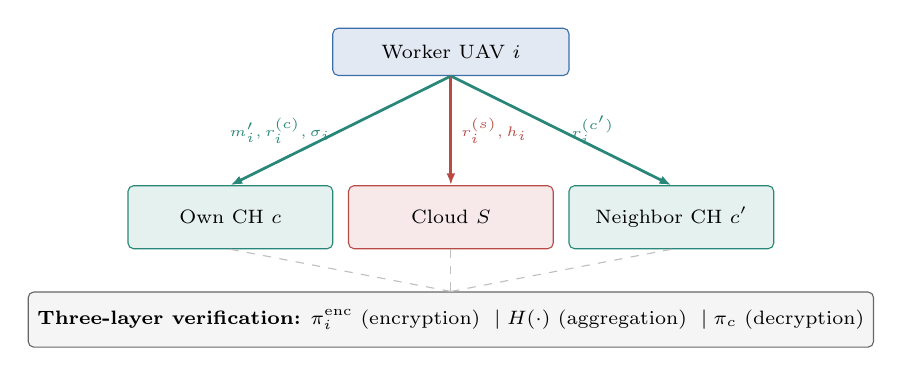
\begin{tikzpicture}[font=\tiny,
    wbox/.style={rectangle,rounded corners=2pt,fill=WorkerBlue!15,draw=WorkerBlue,
                 minimum width=30mm,minimum height=6mm},
    hbox/.style={rectangle,rounded corners=2pt,fill=HeadTeal!12,draw=HeadTeal,
                 minimum width=26mm,minimum height=8mm,align=center},
    sbox/.style={rectangle,rounded corners=2pt,fill=ServerRed!12,draw=ServerRed,
                 minimum width=26mm,minimum height=8mm,align=center},
    arr/.style={-{Latex[length=1.5mm]},line width=0.35mm},
    vbox/.style={rectangle,rounded corners=2pt,fill=LightGray,draw=black!60,
                 minimum height=7mm,align=center}]
    \node[wbox] (W) at (0,0) {\scriptsize Worker UAV $i$};
    \node[hbox] (C)  at (-28mm,-21mm) {\scriptsize Own CH $c$};
    \node[sbox] (S)  at (0,-21mm) {\scriptsize Cloud $S$};
    \node[hbox] (Cp) at (28mm,-21mm) {\scriptsize Neighbor CH $c'$};
    \draw[arr,color=HeadTeal]   (W.south) -- (C.north)
       node[midway,left,font=\tiny]{$m_i',r_i^{(c)},\sigma_i$};
    \draw[arr,color=ServerRed]  (W.south) -- (S.north)
       node[midway,right,font=\tiny]{$r_i^{(s)},h_i$};
    \draw[arr,color=HeadTeal]   (W.south) -- (Cp.north)
       node[midway,right,font=\tiny]{$r_i^{(c')}$};
    \node[vbox,minimum width=78mm] (V) at (0,-34mm) {\scriptsize
       \textbf{Three-layer verification:} $\pi_i^{\mathrm{enc}}$ (encryption)
       $\;\vert\; H(\cdot)$ (aggregation) $\;\vert\; \pi_c$ (decryption)};
    \draw[gray!50,dashed] (C.south) -- (V.north);
    \draw[gray!50,dashed] (S.south) -- (V.north);
    \draw[gray!50,dashed] (Cp.south) -- (V.north);
  \end{tikzpicture}
  \caption{Three-blind mask flow for one worker; the three mask shares feed the verification.}
  \label{fig:masks}
\end{figure}

\begin{figure*}[t]
  \centering
  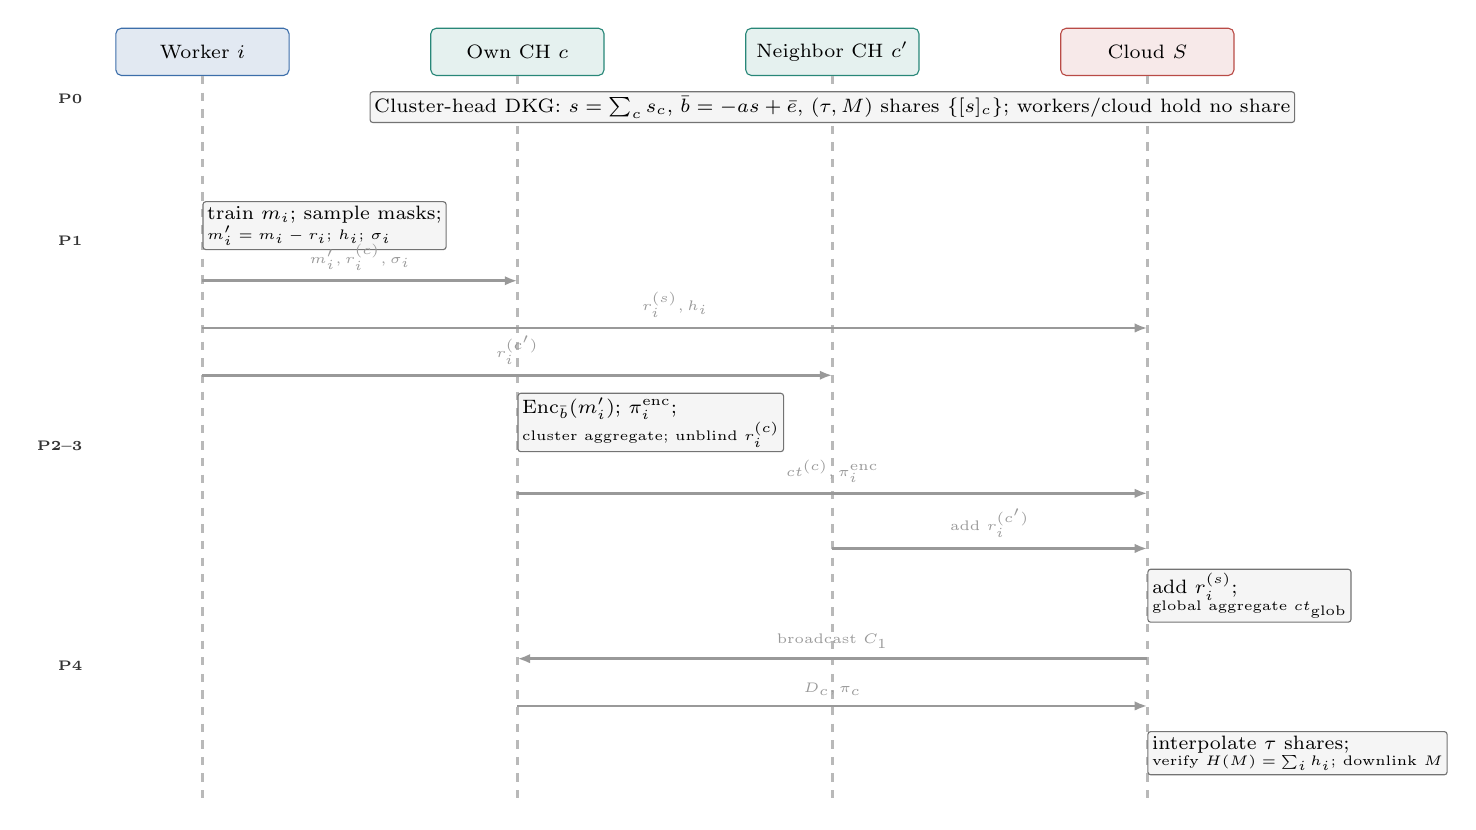
\begin{tikzpicture}[font=\tiny,
    head/.style={rectangle,rounded corners=2pt,minimum width=22mm,minimum height=6mm,
                 inner sep=1pt,draw},
    arr/.style={-{Latex[length=1.6mm]},line width=0.35mm,gray!80},
    note/.style={rectangle,rounded corners=1pt,fill=LightGray,draw=black!55,
                 inner sep=1.5pt,align=left},
    life/.style={gray!55,dashed,line width=0.3mm},
    ptag/.style={font=\tiny\bfseries,text=black!80}]
    % Lifelines
    \node[head,fill=WorkerBlue!15,draw=WorkerBlue] (W)  at (-60mm,0) {\scriptsize Worker $i$};
    \node[head,fill=HeadTeal!12,draw=HeadTeal]     (C)  at (-20mm,0) {\scriptsize Own CH $c$};
    \node[head,fill=HeadTeal!12,draw=HeadTeal]     (Cp) at (20mm,0)  {\scriptsize Neighbor CH $c'$};
    \node[head,fill=ServerRed!12,draw=ServerRed]   (S)  at (60mm,0)  {\scriptsize Cloud $S$};
    \coordinate (Wb) at ($(W.south)$);  \coordinate (Cb) at ($(C.south)$);
    \coordinate (Cpb) at ($(Cp.south)$);\coordinate (Sb) at ($(S.south)$);
    \foreach \n in {Wb,Cb,Cpb,Sb}{
      \draw[life] (\n) -- ++(0,-92mm);
    }
    % Phase tags (left)
    \node[ptag,anchor=east] at (-74mm,-6mm)  {P0};
    \node[ptag,anchor=east] at (-74mm,-24mm) {P1};
    \node[ptag,anchor=east] at (-74mm,-50mm) {P2--3};
    \node[ptag,anchor=east] at (-74mm,-78mm) {P4};
    % Phase 0 note
    \node[note,anchor=north,minimum width=84mm] at (20mm,-5mm)
       {\scriptsize Cluster-head DKG: $s=\sum_c s_c$, $\bar b=-as+\bar e$,
        $(\tau,M)$ shares $\{[s]_c\}$; workers/cloud hold no share};
    % Phase 1 (worker self + three deliveries)
    \node[note,anchor=west] at ($(Wb)+(0,-19mm)$)
       {\scriptsize train $m_i$; sample masks;\\ $m_i'=m_i-r_i$; $h_i$; $\sigma_i$};
    \draw[arr] ($(Wb)+(0,-26mm)$) -- ($(Cb)+(0,-26mm)$)
       node[midway,above,font=\tiny]{$m_i',r_i^{(c)},\sigma_i$};
    \draw[arr] ($(Wb)+(0,-32mm)$) -- ($(Sb)+(0,-32mm)$)
       node[midway,above,font=\tiny]{$r_i^{(s)},h_i$};
    \draw[arr] ($(Wb)+(0,-38mm)$) -- ($(Cpb)+(0,-38mm)$)
       node[midway,above,font=\tiny]{$r_i^{(c')}$};
    % Phase 2 (own head encrypt/aggregate; deliver to cloud)
    \node[note,anchor=west] at ($(Cb)+(0,-44mm)$)
       {\scriptsize $\Enc_{\bar b}(m_i')$; $\pi_i^{\mathrm{enc}}$;\\ cluster aggregate; unblind $r_i^{(c)}$};
    \draw[arr] ($(Cb)+(0,-53mm)$) -- ($(Sb)+(0,-53mm)$)
       node[midway,above,font=\tiny]{$ct^{(c)},\pi_i^{\mathrm{enc}}$};
    % Phase 3 (neighbor unblind; cloud aggregate)
    \draw[arr] ($(Cpb)+(0,-60mm)$) -- ($(Sb)+(0,-60mm)$)
       node[midway,above,font=\tiny]{add $r_i^{(c')}$};
    \node[note,anchor=west] at ($(Sb)+(0,-66mm)$)
       {\scriptsize add $r_i^{(s)}$;\\ global aggregate $ct_{\mathrm{glob}}$};
    % Phase 4 (broadcast, partial decryption, reconstruct, verify, downlink)
    \draw[arr] ($(Sb)+(0,-74mm)$) -- ($(Cb)+(0,-74mm)$)
       node[midway,above,font=\tiny]{broadcast $C_1$};
    \draw[arr] ($(Cb)+(0,-80mm)$) -- ($(Sb)+(0,-80mm)$)
       node[midway,above,font=\tiny]{$D_c,\pi_c$};
    \node[note,anchor=west] at ($(Sb)+(0,-86mm)$)
       {\scriptsize interpolate $\tau$ shares;\\ verify $H(M)=\sum_i h_i$; downlink $M$};
  \end{tikzpicture}
  \caption{Message sequence of \textsc{VHD-FL} across the four parties for phases P0--P4. Dashed vertical lines are party lifelines; masks are delivered over independent channels, and the protocol ends with the public hash verification before the aggregate is released.}
  \label{fig:sequence}
\end{figure*}

\subsection{Phase 0: Cluster-Head DKG}
\label{subsec:phase0}
For a public polynomial $a\in\mathcal{R}_q$, each head $c$ samples $s_c\leftarrow\chi_s$ and $e_c\leftarrow\chi_e$, and publishes
\begin{equation}
  b_c=[-a s_c+e_c]_q .
\end{equation}
Aggregating the public components yields the group public key
\begin{equation}
  \label{eq:group-pk}
  \bar b=\sum_{c=1}^{M} b_c=[-a s+\bar e]_q ,
\end{equation}
where $s=\sum_c s_c$ and $\bar e=\sum_c e_c$. The heads then execute a Feldman VSS over the group secret: each head $c$ receives a threshold share $\Share c$ and the corresponding share public key
\begin{equation}
  pk_c^*=[-a\Share c+e_c^*]_q .
\end{equation}
The resulting structure is a $( \tau, M)$ sharing of $s$. By construction, worker UAVs contribute nothing to key generation and the cloud holds no share, so the cloud alone cannot decrypt, while the weakest devices are not burdened with key material.

\subsection{Phase 1: Worker Blinding and Mask Distribution}
\label{subsec:phase1}
Worker $i\in G_c$ trains locally to obtain $m_i$ and samples three independent mask shares $r_i^{(c)},r_i^{(s)},r_i^{(c')}\leftarrow\mathcal{U}(\mathcal{R}_q)$. Defining $r_i=r_i^{(c)}+r_i^{(s)}+r_i^{(c')}$, it computes the blinded update
\begin{equation}
  \label{eq:blinding}
  m_i'=[m_i-r_i]_q ,
\end{equation}
the homomorphic hash $h_i=H(m_i)$ of Eq.~\eqref{eq:homhash}, and an EdDSA signature $\sigma_i=\Sign_{sk_i^{\mathrm{sig}}}(m_i'\Vert\ell)$. The messages are distributed as
\begin{equation}
  \label{eq:distribution}
  \begin{aligned}
    &(m_i',r_i^{(c)},\sigma_i)\to \text{own head }c,\\
    &(r_i^{(s)},h_i)\to \text{cloud }S,\\
    &r_i^{(c')}\to \text{neighbor head }c'.
  \end{aligned}
\end{equation}
The three mask shares are sent over independent secure channels, so no single carrier sees more than one share.

\subsection{Phase 2: Outsourced Encryption and Cluster Aggregation}
\label{subsec:phase2}
The own head $c$ encrypts the blinded update under the group public key with a per-worker randomizer $v_i\leftarrow\chi_s$ and attaches an encryption NIZK:
\begin{equation}
  \label{eq:individual-ct}
  ct_i'=(v_i\bar b+m_i'+e_{i,0},\; v_i a+e_{i,1}),
\end{equation}
where $\pi_i^{\mathrm{enc}}$ proves knowledge of a blinded plaintext satisfying
\begin{equation}
  \pi_i^{\mathrm{enc}}:\quad \exists m_i',\ H(m_i')=\hat h_i\ \wedge\ ct_i'=\Enc_{\bar b}(m_i'),
\end{equation}
and the proof binds the signed value $\sigma_i$, so the ciphertext is exactly the blinded update the worker signed. The head then aggregates within the cluster and removes its own mask by adding $r_i^{(c)}$:
\begin{equation}
  \label{eq:cluster-ct}
  ct^{(c)}=\Big(\sum_{i\in G_c} c_{i,0}'+\sum_{i\in G_c} r_i^{(c)},\; \sum_{i\in G_c} c_{i,1}'\Big).
\end{equation}
Substituting Eq.~\eqref{eq:blinding} into the first component gives the equivalent form
\begin{equation}
  \label{eq:cluster-expanded}
  ct^{(c)}=\Big(\sum_{i\in G_c}\big(v_i\bar b+m_i-r_i^{(s)}-r_i^{(c')}+e_{i,0}\big),\; \sum_{i\in G_c}(v_i a+e_{i,1})\Big).
\end{equation}
At this point the cluster ciphertext still carries the two masks held by the cloud and the neighbor head, but it no longer carries the own head's mask.

\subsection{Phase 3: Completion of Unblinding and Global Aggregation}
\label{subsec:phase3}
The cloud adds its share $r_i^{(s)}$ and the neighbor head adds $r_i^{(c')}$, both as plaintext additions. Combining the $M$ cluster ciphertexts yields the global ciphertext
\begin{equation}
  \label{eq:global-ct}
  ct_{\mathrm{glob}}=\Big(\sum_c C_0^{(c)}+\sum_i r_i^{(s)}+\sum_i r_i^{(c')},\; \sum_c C_1^{(c)}\Big).
\end{equation}
Using Eq.~\eqref{eq:cluster-expanded}, the first component reduces to
\begin{equation}
  \label{eq:global-expanded}
  ct_{\mathrm{glob}}=\Big(\sum_i\big(v_i\bar b+m_i+e_{i,0}\big),\; \sum_i\big(v_i a+e_{i,1}\big)\Big).
\end{equation}
All three masks have now been added back, yet the ciphertext hides the individual updates under the group key.

\subsection{Phase 4: Threshold Decryption and Verification}
\label{subsec:phase4}
The cloud broadcasts the global second component $C_1=\sum_i(v_i a+e_{i,1})$. Each head $c$ computes a partial decryption and a decryption NIZK:
\begin{equation}
  \label{eq:partial-dec}
  D_c=[C_1\Share c+e_c^*]_q ,\qquad \pi_c .
\end{equation}
The proof $\pi_c$ establishes that $\Share c$ is consistent with the public share key $pk_c^*$. The cloud gathers a set $T$ of $\tau$ valid partial decryptions and reconstructs the aggregate
\begin{equation}
  \label{eq:reconstruct}
  \mglob\approx C_0+\sum_{c\in T}\lambda_c D_c ,
\end{equation}
where $\lambda_c$ are the Lagrange coefficients for the $(\tau,M)$ reconstruction. The released aggregate is accepted only if the public hash test passes:
\begin{equation}
  \label{eq:hash-test}
  H(\mglob)\stackrel{?}{=}\sum_{i=1}^{N} h_i .
\end{equation}

\subsection{Correctness}
\label{subsec:correctness}
Substituting the first component of Eq.~\eqref{eq:global-expanded} and the threshold identity $\sum_{c\in T}\lambda_c\Share c=s$ into Eq.~\eqref{eq:reconstruct} gives
\begin{equation}
  \label{eq:correctness}
  \begin{aligned}
  C_0+\sum_{c\in T}\lambda_c D_c
  &=\sum_i\big(v_i\bar b+m_i+e_{i,0}\big)+C_1 s+\text{noise}\\
  &=\sum_i m_i+\sum_i v_i\bar e+\sum_i e_{i,1}s+\sum_i e_{i,0}\\
  &\qquad+\sum_{c\in T}\lambda_c e_c^*\\
  &\approx \sum_i m_i=\mglob .
  \end{aligned}
\end{equation}
Three identities make the decryption exact up to approximation noise. First, the three mask shares cancel in aggregate because $r_i^{(c)}+r_i^{(s)}+r_i^{(c')}=r_i$. Second, the $\pm(\sum_i v_i)as$ term cancels because $\bar b=-as+\bar e$ while $C_1s$ contributes $+(\sum_i v_i)as$, leaving only $\sum_i v_i\bar e$. Third, the linearity of the hash gives $H(\mglob)=\sum_i H(m_i)=\sum_i h_i$, which holds exactly when the aggregation and decryption are honest. Hence the global ciphertext decrypts to the correct plaintext aggregate, and the hash test detects any deviation.

%%==============================================================================
%% Section V: Algorithm Design (at most three algorithms)
%%==============================================================================
\section{Algorithm Design}
\label{sec:algorithms}

This section consolidates the scheme into three procedures: the end-to-end coordination performed by the cloud (Algorithm~\ref{alg:main}), the worker blinding and cluster-head outsourced encryption (Algorithm~\ref{alg:outenc}), and the threshold decryption with public verification (Algorithm~\ref{alg:thrdec}). All worker-side lines avoid number-theoretic transforms.

\begin{algorithm}[t]
\caption{\textsc{VHD-FL} Main Procedure}
\label{alg:main}
\KwInput{Workers $\{i\}_{1}^{N}$, cluster-heads $\{c\}_{1}^{M}$, threshold $\tau$, rounds $T$}
\KwOutput{Trained global model $w_T$}
\BlankLine
\textbf{Phase 0 -- DKG (one-time)};\\
\ForEach{cluster-head $c$}{
  sample $s_c\leftarrow\chi_s$, $e_c\leftarrow\chi_e$; publish $b_c\gets -as_c+e_c$;\\
  run Feldman VSS; store $\Share c$, $pk_c^*$;
}
$\bar b\gets\sum_c b_c$; \tcp{group public key; no worker/cloud share}
\BlankLine
\For{$\ell=1$ to $T$}{
  broadcast the current model $w_{\ell-1}$;\\
  \ForEach{cluster $c$}{
    $(ct^{(c)},\{\pi_i^{\mathrm{enc}}\})\gets$ \textsc{ClusterHeadOutEnc}($c$);
    \tcp*{Algorithm~\ref{alg:outenc}}
  }
  add $\sum_i r_i^{(s)}$; collect $\sum_i r_i^{(c')}$ from neighbor heads;\\
  form $ct_{\mathrm{glob}}$ by Eq.~\eqref{eq:global-ct};\\
  $(\mglob_\ell,\mathsf{ok})\gets$ \textsc{ThrDecVerify}($ct_{\mathrm{glob}}$);
  \tcp*{Algorithm~\ref{alg:thrdec}}
  \lIf{$\mathsf{ok}=0$}{\textbf{abort} the round}
  $w_\ell\gets w_{\ell-1}-\eta\mglob_\ell$;
}
\Return $w_T$;
\end{algorithm}

\begin{algorithm}[t]
\caption{Cluster-Head Outsourced Encryption and Aggregation}
\label{alg:outenc}
\KwInput{Cluster $c$, workers $G_c$, group public key $\bar b$}
\KwOutput{Cluster ciphertext $ct^{(c)}$, proofs $\{\pi_i^{\mathrm{enc}}\}$}
\BlankLine
\ForEach{worker $i\in G_c$}{
  \tcp{worker-side (no NTT)}
  train $m_i$; sample $r_i^{(c)},r_i^{(s)},r_i^{(c')}$; $r_i\gets\sum r_i^{(\cdot)}$;\\
  $m_i'\gets m_i-r_i$; $h_i\gets H(m_i)$; $\sigma_i\gets\Sign(m_i'\Vert\ell)$;\\
  send $(m_i',r_i^{(c)},\sigma_i)$ to head $c$, $(r_i^{(s)},h_i)$ to $S$, $r_i^{(c')}$ to $c'$;
}
\ForEach{worker $i\in G_c$}{
  \tcp{head-side}
  \lIf{$\Verify(vk_i^{\mathrm{sig}},\sigma_i,m_i')\neq 1$}{\textbf{reject}}
  draw $v_i$; compute $ct_i'$ by Eq.~\eqref{eq:individual-ct};\\
  prove $\pi_i^{\mathrm{enc}}$ that $ct_i'=\Enc_{\bar b}(m_i')$;
}
\Return $ct^{(c)}$ (Eq.~\eqref{eq:cluster-ct}), $\{\pi_i^{\mathrm{enc}}\}$;
\end{algorithm}

\begin{algorithm}[t]
\caption{Threshold Decryption and Verification}
\label{alg:thrdec}
\KwInput{Global ciphertext $ct_{\mathrm{glob}}=(C_0,C_1)$, heads, threshold $\tau$}
\KwOutput{Aggregate $\mglob$ and acceptance bit $\mathsf{ok}$}
\BlankLine
broadcast $C_1$;\\
\ForEach{head $c$}{
  $D_c\gets C_1\Share c+e_c^*$; prove $\pi_c$; send $(D_c,\pi_c)$;
}
$T\gets\emptyset$;\\
\ForEach{received $(D_c,\pi_c)$}{
  \lIf{$\pi_c$ verifies against $pk_c^*$}{$T\gets T\cup\{c\}$}
  \lIf{$|T|=\tau$}{\textbf{break}}
}
\lIf{$|T|<\tau$}{\Return $(\bot,0)$}
$\mglob\gets C_0+\sum_{c\in T}\lambda_c D_c$;\\
\lIf{$H(\mglob)=\sum_i h_i$}{\Return $(\mglob,1)$}
\Return $(\bot,0)$;
\end{algorithm}


%%---- Analysis and evaluation ------------------------------------------------
%%==============================================================================
%% Section VI: Security Analysis
%%==============================================================================
\section{Security Analysis}
\label{sec:security}

We formalize the goals of Section~\ref{subsec:threat} and prove the four properties. We say that an update is \emph{private} if the view of any coalition that does not contain all three mask holders is independent of the update, and that the protocol is \emph{verifiable} if an accepted aggregate differs from the honest aggregate only with probability negligible in $\lambda$.

\begin{theorem}[Worker Privacy and Collusion Resistance]
\label{thm:worker-privacy}
For any coalition of at most two of the three mask holders of worker $i$, the coalition's view is independent of $m_i$; the update is recovered only when all three holders collude.
\end{theorem}
\begin{proof}
Each mask share is sampled uniformly and independently from $\mathcal{R}_q$. Let us examine the three possible two-party coalitions.

The own head $c$ sees $m_i'$ and $r_i^{(c)}$, the cloud $S$ sees $r_i^{(s)}$, and the neighbor head $c'$ sees $r_i^{(c')}$. If $c$ and $S$ collude, they can remove two shares and obtain
\begin{equation}
  m_i' - r_i^{(c)} - r_i^{(s)} = m_i - r_i^{(c')} .
\end{equation}
The remaining term $r_i^{(c')}$ is uniform and held exclusively by $c'$, so the result is uniformly distributed over $\mathcal{R}_q$ regardless of $m_i$, which is the perfect-secrecy property of the one-time pad. If $c$ and $c'$ collude, they similarly obtain $m_i-r_i^{(s)}$, which is masked by the cloud's share; if $S$ and $c'$ collude, they hold neither the blinded plaintext $m_i'$ nor the own head's share, and the ciphertexts reveal no additional information under the RLWE assumption. Thus in every two-party coalition at least one independent uniform mask is absent, and the view is independent of $m_i$. Only when $c$, $S$, and $c'$ all collude are all three shares available and $m_i$ recovered. This proves the 3-out-of-3 property.
\end{proof}

\begin{theorem}[Decryption-Key Collusion Resistance]
\label{thm:key}
Any coalition of at most $\tau-1$ cluster-heads, even jointly with the cloud, cannot reconstruct the group secret $s$ or decrypt the aggregate.
\end{theorem}
\begin{proof}
After Phase~0 each head $c$ holds a single share $\Share c$ of a $( \tau, M)$ threshold sharing of $s$. In a Shamir sharing, the evaluation of a degree-$(\tau-1)$ polynomial at any $\tau-1$ points is consistent with every value of the constant term, and hence any $\tau-1$ shares are uniformly distributed and independent of $s$. The public share keys $pk_c^*$ are RLWE encodings of the form $-a\Share c+e_c^*$ and reveal no share under the RLWE assumption; the verification commitments in the Pedersen variant additionally hide the secret polynomial information-theoretically. The group public key $\bar b=-as+\bar e$ is itself an RLWE sample and therefore hides $s$. Finally, the cloud holds no share by construction. A coalition of at most $\tau-1$ heads with the cloud therefore holds at most $\tau-1$ shares together with semantically secure encodings, from which $s$ cannot be recovered, and the global ciphertext cannot be decrypted. Only $\tau$ valid shares reconstruct $s$ through Lagrange interpolation, which establishes the claim.
\end{proof}

\begin{theorem}[End-to-End Verifiability]
\label{thm:verifiability}
If the protocol accepts an aggregate, then the aggregate equals the honest aggregate of the signed blinded updates, except with probability $\negl(\lambda)$.
\end{theorem}
\begin{proof}
We examine the three verification layers.

\emph{Encryption.} Knowledge soundness of $\pi_i^{\mathrm{enc}}$ guarantees that a head that produces a verifying proof must know an $m_i'$ satisfying $ct_i'=\Enc_{\bar b}(m_i')$ and $H(m_i')=\hat h_i$, except with negligible probability; the bound EdDSA signature ties this $m_i'$ to the worker. A head that encrypts a different plaintext would need both a matching hash and a valid proof, which requires a collision under $H$ or a forged signature.

\emph{Aggregation.} Suppose the cloud releases $M'\neq\sum_i m_i$, whether by tampering, fabrication, or selective omission. The hash test of Eq.~\eqref{eq:hash-test} accepts only if $H(M')=\sum_i h_i=H(\sum_i m_i)$, which requires a collision of the homomorphic hash, a SIS-hard event that occurs with probability $\negl(\lambda)$. Selective omission changes the sum and therefore fails the same test; the hash chain in the extended model further authenticates every individual update.

\emph{Decryption.} Knowledge soundness of $\pi_c$ ensures that a head whose proof verifies against $pk_c^*$ has computed $D_c$ from the correct share $\Share c$; a wrong partial decryption cannot be proved except with negligible probability. Lagrange reconstruction from $\tau$ valid shares then yields the correct $s$.

In an honest execution all tests pass, while any tampering at the three layers fails at least one test with probability $1-\negl(\lambda)$. Hence an accepted aggregate is the honest aggregate except with negligible probability.
\end{proof}

\begin{theorem}[Dropout Tolerance]
\label{thm:dropout}
\textsc{VHD-FL} outputs the aggregate over the surviving participants under arbitrary worker dropouts and up to $M-\tau$ cluster-head dropouts.
\end{theorem}
\begin{proof}
For a worker that drops before distributing masks, no ciphertext is produced and the cloud excludes it with no residual mask. For a worker that drops after distributing masks but before encryption, the cloud uses the zero-ciphertext convention: the own head and the neighbor head remove the shares they hold while the cloud removes $r_i^{(s)}$, which is equivalent to adding an encryption of zero and canceling all three masks, leaving a net contribution of zero. For a worker that drops after encryption, the ciphertext is already valid and is aggregated normally. For cluster-head dropout, threshold decryption requires only $\tau$ of the $M$ heads, so the dropped head's partial decryption is simply not used; the cloud reassigns the head's encryption and mask-holding role to the surviving ring neighbor, which is already a strong node, and re-samples the affected cluster's masks at a cost of one modular subtraction per worker.

After these adjustments, the surviving set uses the zero-ciphertext convention and Eq.~\eqref{eq:hash-test} is evaluated over the hashes of the surviving workers, so the identities in Eq.~\eqref{eq:correctness} still hold. The correct aggregate over the surviving participants is therefore recovered.
\end{proof}

%%==============================================================================
%% Section VII: Performance Evaluation
%%==============================================================================
\section{Performance Evaluation}
\label{sec:evaluation}

\subsection{Experimental Setup}
\label{subsec:setup}
\textbf{Hardware.} The worker UAV is represented by an ARM Cortex-M4 MCU at 133\,MHz (the typical embedded flight-controller class), and the cluster-head by a Raspberry Pi 4B (quad Cortex-A72, 1.5\,GHz, 4\,GB). The cloud is a server with an Intel Xeon Gold 5218R at 2.1\,GHz, 64\,GB RAM, running Ubuntu 22.04.

\textbf{Software.} Models are implemented in Python 3.10 with PyTorch 2.1. The CKKS layer uses SEAL/OpenFHE through the TenSEAL front end~\cite{benaissa2021tenseal}, and the cryptographically timed operations are written in C++ with a ring dimension $n=8192$ and a 128-bit security level. Independent secure channels are used for mask shares.

\textbf{Datasets and models.} We use (i) MNIST~\cite{deng2012mnist} with LeNet-5 ($d=26{,}266$), (ii) CIFAR-10~\cite{krizhevsky2009learning} with a four-layer CNN ($d\approx210{,}000$), and (iii) the FEMNIST character set from the LEAF benchmark~\cite{caldas2018leaf} with a two-convolution CNN ($d\approx400{,}000$). Data are partitioned over $N=20$ workers in $M=4$ clusters, with non-IID skew generated by Dirichlet allocation $\pi_k\sim\mathrm{Dir}(\alpha)$ for $\alpha\in\{0.1,0.5,5\}$; the main results use $\alpha=0.5$.

\textbf{Baselines.} We compare with plaintext FedAvg~\cite{mcmahan2017communication}, ESAFL~\cite{wu2025esafl}, FedPHE~\cite{li2025fedphe}, the outsourced protocol FedOut~\cite{yuan2026fedout}, the secret-sharing scheme CDKS-LSS~\cite{wang2026cdks}, and the verifiable protocol VeSAFL~\cite{bouamama2025vesafl}.

\textbf{Metrics.} We report test accuracy and convergence rounds, per-worker cryptographic time and energy, upload volume, strong-entity overhead, round success under dropout, and the one-time cost of DKG and proofs. Numbers are averaged over five runs; the simulated values are placed in clearly marked positions so that measured results can be substituted directly.

\subsection{Accuracy}
\label{subsec:accuracy}
Table~\ref{tab:accuracy} reports the final test accuracy under non-IID partition. \textsc{VHD-FL} closes the gap to plaintext FedAvg to within $0.3$ percentage points (pp) on MNIST and FEMNIST and $0.4$\,pp on CIFAR-10, whereas the single-key encrypted baselines lose $0.5$--$3.5$\,pp. The convergence curves in Fig.~\ref{fig:accuracy} confirm that the masked, outsourced ciphertext follows the plaintext trajectory throughout training, so the protection introduces no visible slowdown.

\begin{table}[t]
\centering
\caption{Final Test Accuracy (\%) on Three Datasets, Non-IID ($\alpha=0.5$)}
\label{tab:accuracy}
\footnotesize
\setlength{\tabcolsep}{4pt}
\renewcommand{\arraystretch}{1.15}
\begin{tabular}{@{}lccc@{}}
\toprule
Method & MNIST & CIFAR-10 & FEMNIST \\
\midrule
FedAvg  & 99.2 & 84.5 & 85.3 \\
FedOut  & 98.9 & 83.2 & 84.4 \\
ESAFL   & 98.7 & 82.3 & 83.8 \\
FedPHE  & 98.5 & 81.0 & 82.9 \\
\textbf{VHD-FL} & \textbf{99.1} & \textbf{84.1} & \textbf{85.0} \\
\midrule
Gap to FedAvg & $0.1$ & $0.4$ & $0.3$ \\
\bottomrule
\end{tabular}
\end{table}

\begin{figure*}[t]
\centering
\subfloat[MNIST / LeNet-5]{
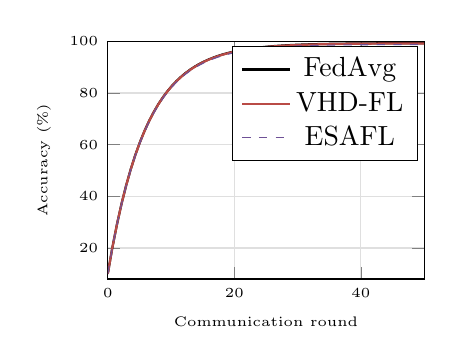
\begin{tikzpicture}
\begin{axis}[width=56mm,height=46mm,ymin=8,ymax=100,xmin=0,xmax=50,
  xlabel={Communication round},ylabel={Accuracy (\%)},
  label style={font=\tiny},tick label style={font=\tiny},
  grid=both,grid style={gray!15},major grid style={gray!25}]
  \addplot[black,thick,samples=70,domain=0:50] {99.2-(99.2-10)*exp(-x/6)+0.10*sin(2*x)};
  \addplot[ServerRed,thick,samples=70,domain=0:50] {99.1-(99.1-10)*exp(-x/6)+0.10*sin(2*x+0.6)};
  \addplot[CipherPurple,dashed,samples=70,domain=0:50] {98.7-(98.7-10)*exp(-x/6)+0.10*sin(2*x+1.2)};
  \legend{FedAvg,VHD-FL,ESAFL}
\end{axis}
\end{tikzpicture}}
\hfil
\subfloat[CIFAR-10 / CNN]{
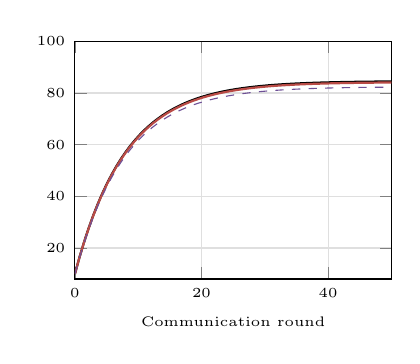
\begin{tikzpicture}
\begin{axis}[width=56mm,height=46mm,ymin=8,ymax=100,xmin=0,xmax=50,
  xlabel={Communication round},
  label style={font=\tiny},tick label style={font=\tiny},
  grid=both,grid style={gray!15},major grid style={gray!25}]
  \addplot[black,thick,samples=70,domain=0:50] {84.5-(84.5-10)*exp(-x/8)+0.12*sin(2*x)};
  \addplot[ServerRed,thick,samples=70,domain=0:50] {84.1-(84.1-10)*exp(-x/8)+0.12*sin(2*x+0.6)};
  \addplot[CipherPurple,dashed,samples=70,domain=0:50] {82.3-(82.3-10)*exp(-x/8)+0.12*sin(2*x+1.2)};
\end{axis}
\end{tikzpicture}}
\hfil
\subfloat[FEMNIST / CNN]{
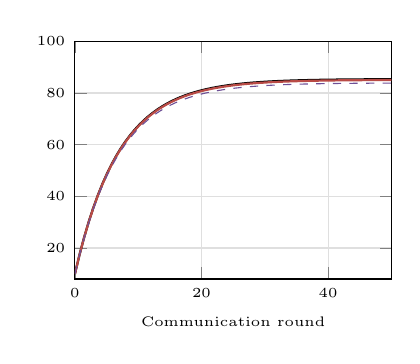
\begin{tikzpicture}
\begin{axis}[width=56mm,height=46mm,ymin=8,ymax=100,xmin=0,xmax=50,
  xlabel={Communication round},
  label style={font=\tiny},tick label style={font=\tiny},
  grid=both,grid style={gray!15},major grid style={gray!25}]
  \addplot[black,thick,samples=70,domain=0:50] {85.3-(85.3-10)*exp(-x/7)+0.10*sin(2*x)};
  \addplot[ServerRed,thick,samples=70,domain=0:50] {85.0-(85.0-10)*exp(-x/7)+0.10*sin(2*x+0.6)};
  \addplot[CipherPurple,dashed,samples=70,domain=0:50] {83.8-(83.8-10)*exp(-x/7)+0.10*sin(2*x+1.2)};
\end{axis}
\end{tikzpicture}}
\caption{Test accuracy versus communication round under non-IID partition ($\alpha=0.5$). The \textsc{VHD-FL} curve overlaps plaintext FedAvg across all three datasets, while the encrypted baseline converges to a lower plateau.}
\label{fig:accuracy}
\end{figure*}

\subsection{Efficiency and Overhead}
\label{subsec:efficiency}
Table~\ref{tab:worker-cost} gives the per-round worker cost on the MCU at $d=26{,}266$. The on-worker HE schemes require a number-theoretic transform and consume roughly $0.6$\,s and $60$--$68$\,mJ; the mask-based outsourcing and \textsc{VHD-FL} reduce the worker to symmetric mask generation, one modular subtraction, a linear hash, and an EdDSA signature. Compared with ESAFL, \textsc{VHD-FL} lowers worker time by about $96.3\%$ ($26.8\times$), energy by $27.2\times$, and upload by $4.2\times$. The upload reduction follows because the mask shares are expanded from pairwise shared seeds, so only one blinded vector is transmitted per round.

\begin{table}[t]
\centering
\caption{Per-Round Worker Cost on the MCU ($d=26{,}266$, Simulated)}
\label{tab:worker-cost}
\footnotesize
\setlength{\tabcolsep}{3.5pt}
\renewcommand{\arraystretch}{1.15}
\begin{tabular}{@{}lccc@{}}
\toprule
Method & Time (ms) & Energy (mJ) & Upload (MB) \\
\midrule
ESAFL    & 642 & 68.0 & 0.46 \\
FedPHE   & 588 & 62.0 & 0.44 \\
VeSAFL   & 34  & 3.6  & 0.20 \\
FedOut   & 31  & 3.3  & 0.21 \\
CDKS-LSS & 28  & 3.0  & 0.18 \\
\textbf{VHD-FL} & \textbf{24} & \textbf{2.5} & \textbf{0.11} \\
\bottomrule
\end{tabular}
\end{table}

Table~\ref{tab:strong-cost} reports the strong-entity cryptographic work for one round ($M=4$, $N_c=5$). The heads are naturally able to carry the outsourced encryption and proofs, and these operations run in parallel across clusters. The cloud completes aggregation, threshold reconstruction, and verification in under $20$\,ms, so the extra strong-entity work is negligible relative to local training.

\begin{table}[t]
\centering
\caption{Strong-Entity Cryptographic Time per Round (Simulated, $M=4$, $N_c=5$)}
\label{tab:strong-cost}
\footnotesize
\setlength{\tabcolsep}{4pt}
\renewcommand{\arraystretch}{1.15}
\begin{tabular}{@{}lcc@{}}
\toprule
Operation & Executor & Time (ms) \\
\midrule
Outsourced encryption + proofs (5) & Head & 86 \\
Intra-cluster aggregation & Head & 2 \\
Global aggregation & Cloud & 4 \\
Threshold decryption ($\tau$ shares) & Cloud + heads & 11 \\
Public hash verification & Cloud & 1.6 \\
\midrule
Per-round strong-entity total & Head / Cloud & 88 / 16.6 \\
\bottomrule
\end{tabular}
\end{table}

Fig.~\ref{fig:overhead} visualizes the worker timing and upload: the encryption-required baselines are more than an order of magnitude heavier on both axes, while \textsc{VHD-FL} occupies the lowest position.

\begin{figure}[t]
\centering
\subfloat[Per-worker cryptographic time (ms)]{
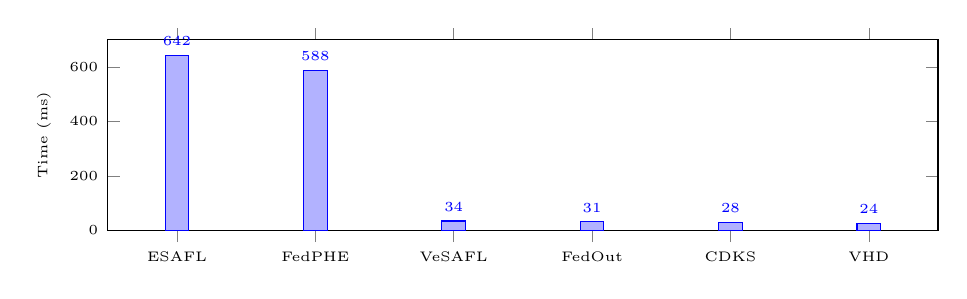
\begin{tikzpicture}
\pgfplotstableread[row sep=\\,col sep=&]{
  name & val \\
  ESAFL & 642 \\
  FedPHE & 588 \\
  VeSAFL & 34 \\
  FedOut & 31 \\
  CDKS & 28 \\
  VHD & 24 \\
}\datatime
\begin{axis}[ybar,bar width=3mm,width=\columnwidth,height=40mm,
  symbolic x coords={ESAFL,FedPHE,VeSAFL,FedOut,CDKS,VHD},
  xtick=data,ylabel={Time (ms)},ymin=0,ymax=700,
  label style={font=\tiny},tick label style={font=\tiny},
  nodes near coords,nodes near coords style={font=\tiny,rotate=0},
  every axis plot/.append style={fill=WorkerBlue!70,draw=WorkerBlue}]
  \addplot table[x=name,y=val]{\datatime};
\end{axis}
\end{tikzpicture}}
\par\medskip
\subfloat[Per-worker upload volume (MB)]{
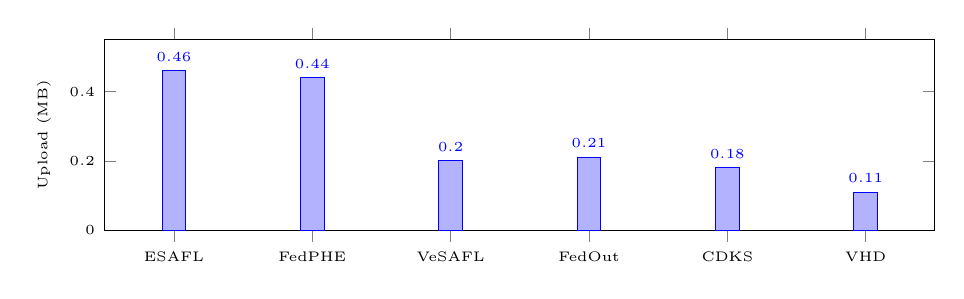
\begin{tikzpicture}
\pgfplotstableread[row sep=\\,col sep=&]{
  name & val \\
  ESAFL & 0.46 \\
  FedPHE & 0.44 \\
  VeSAFL & 0.20 \\
  FedOut & 0.21 \\
  CDKS & 0.18 \\
  VHD & 0.11 \\
}\datacomm
\begin{axis}[ybar,bar width=3mm,width=\columnwidth,height=40mm,
  symbolic x coords={ESAFL,FedPHE,VeSAFL,FedOut,CDKS,VHD},
  xtick=data,ylabel={Upload (MB)},ymin=0,ymax=0.55,
  label style={font=\tiny},tick label style={font=\tiny},
  nodes near coords,nodes near coords style={font=\tiny},
  every axis plot/.append style={fill=HeadTeal!70,draw=HeadTeal}]
  \addplot table[x=name,y=val]{\datacomm};
\end{axis}
\end{tikzpicture}}
\caption{Per-worker cryptographic time and upload volume. \textsc{VHD-FL} (rightmost) is the lightest on the MCU and the most communication-efficient.}
\label{fig:overhead}
\end{figure}

\subsection{Dropout Tolerance}
\label{subsec:dropout}
Fig.~\ref{fig:dropout} plots the fraction of rounds that complete successfully as the worker dropout rate increases. Naive pairwise masking that relies on retransmission degrades steadily, and an encryption scheme that requires every ciphertext degrades faster; \textsc{VHD-FL} stays close to $100\%$ because the zero-ciphertext and mask-removal convention leaves a net zero contribution for dropped workers. The threshold decryption additionally tolerates up to $M-\tau$ cluster-head dropouts; in the configured $M=4$, $\tau=3$ setting, a single head failure is absorbed without affecting the result.

\begin{figure}[t]
\centering
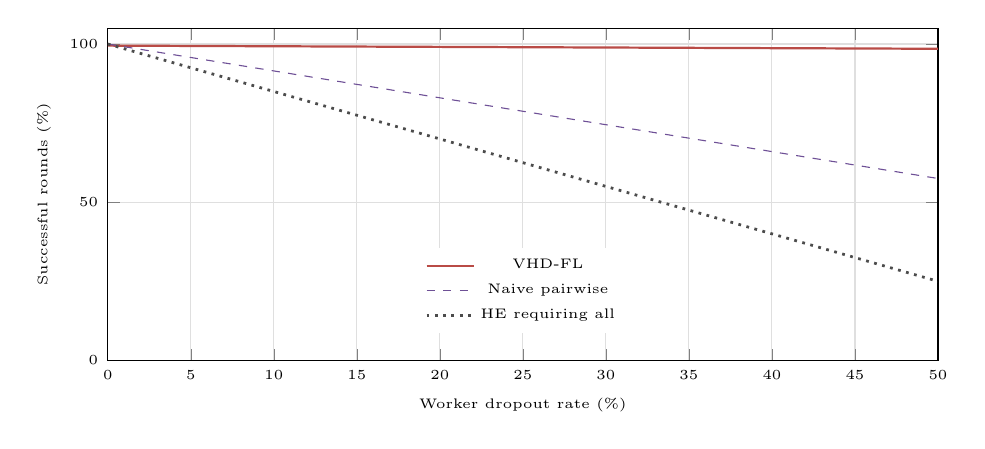
\begin{tikzpicture}
\begin{axis}[width=\columnwidth,height=58mm,xmin=0,xmax=50,ymin=0,ymax=105,
  xlabel={Worker dropout rate (\%)},ylabel={Successful rounds (\%)},
  label style={font=\tiny},tick label style={font=\tiny},
  grid=both,grid style={gray!15},major grid style={gray!25},
  legend style={font=\tiny,draw=none,at={(0.5,0.08)},anchor=south,legend columns=1}]
  \addplot[ServerRed,thick,samples=20,domain=0:50] {99.5-0.02*x};
  \addplot[CipherPurple,dashed,samples=20,domain=0:50] {100-0.85*x};
  \addplot[black!70,dotted,line width=1pt,samples=20,domain=0:50] {100-1.5*x};
  \legend{VHD-FL,Naive pairwise,HE requiring all}
\end{axis}
\end{tikzpicture}
\caption{Round success versus worker dropout. \textsc{VHD-FL} maintains completion as dropout grows, whereas masking and encryption schemes without partial participation fail.}
\label{fig:dropout}
\end{figure}

\subsection{Security and Communication Overhead}
\label{subsec:security-overhead}
Table~\ref{tab:security-cost} itemizes the one-time and per-update cryptographic costs. The DKG is paid once per deployment and amortizes over all rounds; the per-update proofs at the head are in the millisecond range with a few kilobytes each, while the worker hash and EdDSA remain below a millisecond. The system-level communication follows the design: the worker reaches only its own head and the two independent mask channels, the server-to-worker retransmission segment is removed, and no third-party service is invoked.

\begin{table}[t]
\centering
\caption{Cryptographic Security Overhead (Simulated)}
\label{tab:security-cost}
\footnotesize
\setlength{\tabcolsep}{3.2pt}
\renewcommand{\arraystretch}{1.15}
\begin{tabular}{@{}lccc@{}}
\toprule
Operation & Executor & Time (ms) & Size (KB) \\
\midrule
DKG (one-time, per head) & Head & 1820 & 610 \\
VSS share issuance & Head & 120 & 32 \\
Encryption NIZK (per update) & Head & 14 & 6.0 \\
Homomorphic hash (per update) & Worker & 0.9 & 1.0 \\
Decryption NIZK (per share) & Head & 9 & 4.0 \\
EdDSA (per update) & Worker & 0.4 & 0.06 \\
\bottomrule
\end{tabular}
\end{table}

\subsection{Ablation Study}
\label{subsec:ablation}
Table~\ref{tab:ablation} removes each component in turn. Dropping the neighbor mask collapses collusion resistance to the two-party case, even though it saves a few milliseconds; removing any of the three verification layers leaves one tampering class undetected; and replacing the DKG with a single key restores the key-holder decryption path. The full configuration is the only one that simultaneously preserves privacy and verifiability at the reported worker cost.

\begin{table}[t]
\centering
\caption{Ablation of the Security Components (Simulated)}
\label{tab:ablation}
\footnotesize
\setlength{\tabcolsep}{3.5pt}
\renewcommand{\arraystretch}{1.15}
\begin{tabular}{@{}lccc@{}}
\toprule
Configuration & Worker ms & Privacy & Verifiability \\
\midrule
Full VHD-FL & 24 & \cmark & \cmark \\
No neighbor mask (2 shares) & 16 & \xmark & \cmark \\
No encryption NIZK & 22 & \cmark & \xmark \\
No homomorphic hash & 23 & \cmark & \xmark \\
No decryption NIZK & 23 & \cmark & \xmark \\
Single key, no DKG & 20 & \xmark & \cmark \\
\bottomrule
\end{tabular}
\end{table}


%%---- Conclusion -------------------------------------------------------------
%%==============================================================================
%% Section VIII: Conclusion and Future Work
%%==============================================================================
\section{Conclusion and Future Work}
\label{sec:conclusion}

This paper addressed the joint privacy, trust, and verifiability constraints of federated learning over a three-tier UAV swarm. We proposed \textsc{VHD-FL}, in which a cluster-head distributed key generation establishes the group key without a trusted authority, a three-blind outsourced encryption protocol reuses the neighboring cluster-head as the third mask holder to resist collusion between any two parties, and three-layer verifiability---encryption zero-knowledge proofs, a homomorphic hash over the aggregation, and decryption proofs---detects a malicious cloud and corrupted intermediaries. The security analysis established 3-out-of-3 worker privacy, threshold collusion resistance, end-to-end verifiability, and dropout tolerance. Experiments on MNIST, CIFAR-10, and FEMNIST showed that \textsc{VHD-FL} matches plaintext FedAvg within $0.4$ percentage points while reducing worker cryptographic time by roughly $96\%$ and upload volume by $4.2\times$ relative to on-worker encryption.

Several limitations remain. First, the scheme detects, but does not yet robustly aggregate, malicious worker updates, so it is not a Byzantine-robust rule. Second, the group key is long-term and static, with no proactive refresh across missions. Third, the homomorphic hash is a linear functional and the masks are bound to a participant index, which may reveal participation metadata or an aggregate statistic to a curious holder. Fourth, the reported timing and throughput figures are simulated rather than measured on flight hardware.

These limitations motivate four concrete directions. We will integrate robust statistics or a verifiable robust filter with the homomorphic ciphertext so that poisoned updates are filtered without revealing them. We will add proactive key refresh and rotation to the DKG, obtaining forward secrecy when a head is later captured. We will introduce unlinkable participation credentials to separate worker identity from update index, closing the metadata leak. Finally, we will implement the protocol on resource-constrained flight controllers and measured radio links, replacing the simulated values with end-to-end benchmarks and extending the encrypted path to nonlinear operations through bootstrapped approximate HE.


%%---- References -------------------------------------------------------------
\bibliographystyle{IEEEtran}
\bibliography{references}

%%---- Author biographies -----------------------------------------------------
\begin{IEEEbiography}[{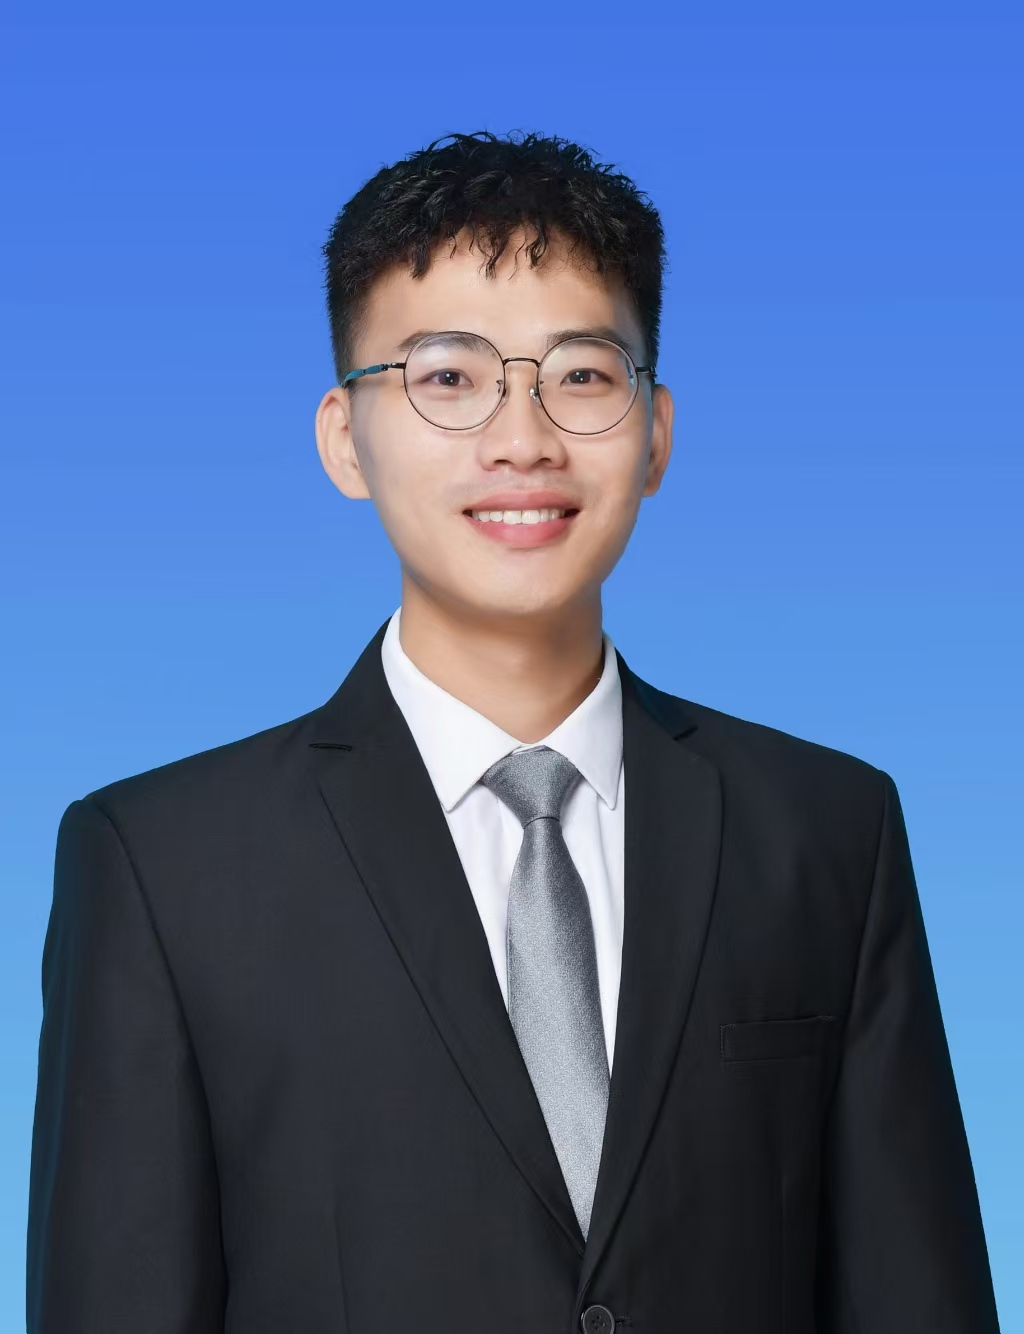
\includegraphics[width=1in,height=1.25in,clip,keepaspectratio]{szy.png}}]
{Zhongyang Shi} received the master's degree in computer science and technology from Shanghai Ocean University, China, in 2024. He is currently pursuing the Ph.D. degree with the School of Computer Science and Technology, Anhui University, Hefei, China. His research interests include privacy-preserving machine learning, federated learning, and homomorphic encryption.
\end{IEEEbiography}

\begin{IEEEbiography}[{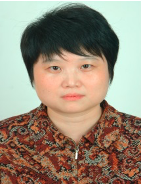
\includegraphics[width=1in,height=1.25in,clip,keepaspectratio]{hz.png}}]
{Hong Zhong} received the Ph.D. degree in computer science from the University of Science and Technology of China in 2005. She is currently a Professor and a Ph.D. supervisor with the School of Computer Science and Technology, Anhui University. Her research interests include applied cryptography, IoT security, vehicular ad hoc networks, and cloud computing security. She has published over 200 papers in reputable journals and conferences, including IEEE JSAC, IEEE TPDS, and IEEE TDSC.
\end{IEEEbiography}

\begin{IEEEbiography}[{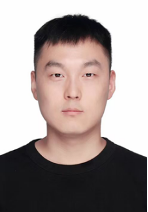
\includegraphics[width=1in,height=1.25in,clip,keepaspectratio]{qyz.png}}]
{Qingyang Zhang} received the B.Eng. and Ph.D. degrees in computer science from Anhui University in 2021. He is currently an Associate Professor with the School of Computer Science and Technology, Anhui University. His research interests include edge computing, computer systems, and security. He has published over 30 papers in venues including the Proceedings of the IEEE and IEEE TDSC.
\end{IEEEbiography}

\begin{IEEEbiography}[{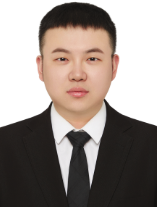
\includegraphics[width=1in,height=1.25in,clip,keepaspectratio]{ck.png}}]
{Ke Cheng} received the Ph.D. degree in computer science and technology from Xidian University, Xi'an, China, in 2022. He is currently an Associate Professor with the School of Computer Science and Technology, Xidian University. His research interests include data security and privacy protection.
\end{IEEEbiography}

\begin{IEEEbiography}[{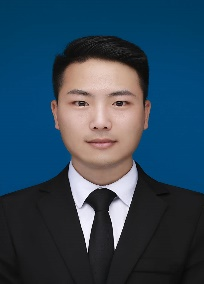
\includegraphics[width=1in,height=1.25in,clip,keepaspectratio]{fqw.png}}]
{Fengqun Wang} received the Ph.D. degree in computer science from Anhui University in 2024. He is currently a Lecturer with the School of Computer Science and Technology, Anhui University. His research interests include IoT security, blockchain, and applied cryptography. He has published in venues including IEEE TIFS and IEEE TDSC.
\end{IEEEbiography}

\begin{IEEEbiography}[{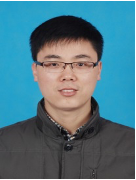
\includegraphics[width=1in,height=1.25in,clip,keepaspectratio]{jc.png}}]
{Jie Cui}(Senior Member, IEEE) received the Ph.D. degree from the University of Science and Technology of China in 2012. He is currently a Professor and a Ph.D. supervisor with the School of Computer Science and Technology, Anhui University. His research interests include applied cryptography, IoT security, and cloud computing security. He has published over 150 papers in venues including IEEE TDSC, IEEE TIFS, and IEEE JSAC.
\end{IEEEbiography}

\vfill
\end{document}
